\documentclass{article}
\usepackage[UTF8]{ctex}
\usepackage{geometry}
\usepackage{natbib}
\geometry{left=3.18cm,right=3.18cm,top=2.54cm,bottom=2.54cm}
\usepackage{graphicx}
\pagestyle{plain}	
\usepackage{setspace}
\usepackage{caption2}
\usepackage{datetime} %日期
\usepackage{float}
\renewcommand{\today}{\number\year 年 \number\month 月 \number\day 日}
\renewcommand{\captionlabelfont}{\small}
\renewcommand{\captionfont}{\small}
\begin{document}

\begin{figure}
    \centering
    
\includegraphics[width=8cm]{upc.png}

    \label{figupc}
\end{figure}

	\begin{center}
		\quad \\
		\quad \\
		\heiti \fontsize{45}{17} \quad \quad \quad 
		\vskip 1.5cm
		\heiti \zihao{2} 《信息技术前沿讲座》课程总结报告
	\end{center}
	\vskip 2.0cm
		
	\begin{quotation}
	%\begin{center}
	\doublespacing
	
	\zihao{4}\par\setlength\parindent{7em}
	\quad 
	
	学生姓名:\underline{\qquad  周新宇 \qquad \qquad}
	
	学\hspace{0.61cm} 号:\underline{\qquad 1808010327\qquad}
	
	专业班级:\underline{\qquad 计算1803 \qquad  }
	
	学\hspace{0.61cm} 院:\underline{计算机科学与技术学院}
	% 	\end{center}
		\vskip 2cm
		\centering
		\begin{table}[h]
            \centering 
            \zihao{4}
            \begin{tabular}{|c|c|c|c|c|c|}
            % 这里的rl 与表格对应可以看到,姓名是r,右对齐的;学号是l,左对齐的;若想居中,使用c关键字。
                \hline
                课程认识 & 问题思 考 & 格式规范  & Latex文档制作   & 总分 & 评阅教师 \\
                30\% & 30\% & 20\% & 20\%  &  &  \\
                \hline
                 & & & &  &\\
                & & & &  &\\
                \hline
            \end{tabular}
        \end{table}
		\vskip 2cm
		\today
	\end{quotation}
\thispagestyle{empty}
\newpage
\setcounter{page}{1}
% 在这之前是封面,在这之后是正文
\section{引言}
随着线上人口和流量红利的终结,中国的移动互联网也在迅速走向成熟。App生态在趋向封闭的同时,出现了严重的马太效应\textsuperscript{\citep{matai1}}。有数据显示,2015年底,国内移动互联网用户规模增长红利消失,进入存量市场的争夺:0.1\%的超级应用占全网分发流量的70\%,意味着中小开发者更难获得流量的倾斜;而且用户安装应用的兴趣低迷,50\%的用户月安装应用数为0,新的应用更难覆盖到用户。在这样的背景下,互联网巨头、超级App,甚至包括手机厂商们开始陆续推出无需下载、所见即所得的小程序或类似服务。\textsuperscript{\citep{caibao}}\par
小程序的出现相比于框架更大幅度地降低了应用开发的门槛与周期,这是一种无需下载就能使用的应用。小程序实现了应用的“触手可及”,用户扫一扫或搜一下即可打开应用,体现了“用完即走”的理念,用户无需再担心安装太多应用的问题。经过多年的发展,以微信小程序为代表的小程序家族,已经构造了全新的小程序开发环境和开发者生态。小程序也是这么多年来中国IT行业里一个真正能够影响到普通程序员的创新成果。截至目前,已经有超过150万的开发者加入到了微信小程序的开发,微信小程序的应用数量也超过了一百万,覆盖200多个细分的行业,日活用户达到两个亿。小程序的发展也带来了更多的就业机会,仅发布当年(2017年)小程序就已经带动就业104万人,社会效应不断提升。\textsuperscript{\citep{xcxnumbers}}\par
目前市面上小程序种类众多,虽然使用小程序无需再额外安装新应用,但每种小程序的使用都依赖于某一平台,如微信小程序必须在微信客户端中才可运行,支付宝小程序必须在支付宝客户端中才能运行等。本报告将以最广为人知同时也是占有大部分市场份额\textsuperscript{\citep{xcxfenlei}}的小程序——“微信小程序”为例,以点带面,从技术、发展前景两个角度来展开论述。因为此前在答辩中已着重讲过了小程序的技术特点,所以技术部分仅在此做一个简要回顾,发展前景会在后面做进一步的思考。\par
在技术上,微信为小程序的开发者提供了一个简单、高效的应用开发框架和丰富的组件及API,能够帮助开发者在微信中开发具有原生 APP 体验的服务。同时小程序开发者可以使用云开发开发微信小程序、小游戏。云开发为开发者提供完整的原生云端支持和微信服务支持,弱化后端和运维概念,无需搭建服务器,使用平台提供的API进行核心业务开发,即可实现快速上线和迭代,同时这一能力,同开发者已经使用的云服务相互兼容,并不互斥。\par
为了帮助开发者简单和高效地开发和调试微信小程序,微信在原有的公众号网页调试工具的基础上,推出了全新的微信开发者工具,集成了公众号网页调试和小程序调试两种开发模式。微信官方设计团队和小程序团队还为微信小程序量身设计了一套基于样式库weui-wxss开发的小程序扩展组件库,同微信原生视觉体验一致的UI组件库,令用户的使用感知更加统一。微信还面向小程序开发者、运营者提供了一套数据分析工具来进行小程序数据分析,帮助小程序产品迭代优化和运营。基于微信小程序轻快的特点,微信还拟定了小程序界面设计指南和建议。设计指南建立在充分尊重用户知情权与操作权的基础之上。旨在微信生态体系内,建立友好、高效、一致的用户体验,同时最大程度适应和支持不同需求,实现用户与小程序服务方的共赢。\par
此外,小程序还引入了常见的插件概念,插件是可被添加到小程序内直接使用的功能组件。开发者可以像开发小程序一样开发一个插件,供其他小程序使用。同时,小程序开发者可直接在小程序内使用插件,无需重复开发,为用户提供更丰富的服务。\par
虽然近些年小程序发展势头迅猛,但现有的小程序在庞大的用户市场上还远没有达到需求饱和状态,零售业、生活服务业、游戏娱乐业等几个主产业需求量依然巨大\textsuperscript{\citep{xcxxvqiu}},未来市场将会有更多的小程序被开发和上线,在未来或将迎来新一轮的爆发式发展态势。
\section{对本门课程的认识、体会}
\subsection{总体感受}
通过此门《信息技术前沿讲座》课程,我认识到:整个信息技术产业包括非常多的领域和环节,这是一个高速发展的行业,积累了大量的知识技术,我们在其中成长,犹如逆水行舟,不进则退。同时,在不断学习的过程中,我们更需要在这浩如烟海的知识体系中看清方向,选择好着力点。同时老师结合当下的形式讲解的百年未有之大变局也大大开拓了我的视野。
\par
\subsection{大牛养成指南——do more}
老师在大牛养成指南这部分给我印象最深刻的就是“do more”,感觉这个词一下子点中了我的痛处。身患懒癌的我每天,不仅没有“do more”过,而且时时刻刻都在“do less”。而且很多次睡觉前,盘盘这一天,感觉一整天都坐在电脑前(我电脑上没游戏),但是什么也没做,大部分时间都浪费了。而且回顾一下当天的计划,总是会发现完完全全可以完成的。而且后来发现,其实每次要走神的时候,就在那一个瞬间,就那一瞬间的一个决定,如果那个时间点上允许了自己周神,可能这一下就回不来了,如果当时及时制止住了,可能会专注很久。所以说,认真专注其实也没这么难,而且如果我们能在完成本职工作后,再多做一点点,这就是进取心。多做一点点也许是微不足道的,但是,就是这些微不足道的一点点,会让自身的工作结果发生意想不到的变化。如果每天多做一点点,就有可能变成一名优秀的员工。“每天多做一点点”实际上只要用心,是很容易做到的。其实“每天多做一点点”不仅是要我们多做一些努力,更重要的是要把自己分内的事做的更好。每个人所做的工作都是由一件件小事构成的,但不能因为这些事小而敷衍了事,在完成任务的基础上,再多做一点点,争取做得更好。只有每天多做一点点,才会有丰厚的积累,最终获得回报。
\subsection{演讲选题}
当我第一次看见演讲题目库的时候,我吃惊了好久。一千多个题目,密密麻麻地排列下去。好像发现了一个大宝库一般,顺手搜了几个自己会的或者是道听途说的几门技术,都能搜得到,然后又从头到尾快速地浏览了一遍,深深地感受到了自己的无知,信息技术真的是博大精深。
\section{对演讲题目的进一步的思考}
\subsection{国内小程序市场的70-20-10律}
吴军博士在《浪潮之巅》\textsuperscript{\citep{lczd}}一书中提到过信息产业的一个规律——70-20-10律,其含义为当信息产业中的某个领域发展成熟后(而不是群雄争霸时期),一般容不下三个以上的主要竞争者。这个行业一般有一个老大,它一定会遇到一两个主要的挑战者,也就是老二(也许还有老三)。其余是一大群小商家,老大是这个领域的主导者,不仅占据着超过一半,通常是百分之六七十的市场,并且制定了这个领域的游戏规则。老二有自己稳定的百分之二三十的市场份额,有时也会挑战老大并给老大一些颜色看看,总的来讲是受老大欺负的时间多。剩下的一群小商家数量虽然多,却只能占到10\%甚至更少的市场,基本上唯老大马首是瞻。老大总是密切注视着老二,并时不时地打压它,以防它做大。老大和老二通常都不会太在意剩下的小企业,这样就让这一群小企业有挣一些小钱的地方。这里面的百分比数字70、20和10是作者吴军博士加的,因为信息产业大公司之间的市场份额大抵如此。\par
虽然国内的小程序发展还没有完全成熟,增量市场规模仍然十分值得期待。但是从《互联网周刊》发布的2019年度小程序分类排行\textsuperscript{\citep{xcxfenlei}}上可以看出,微信在小程序市场占有率保持着绝对优势,支付宝紧随其后。
\begin{figure}[H]
	\centering
	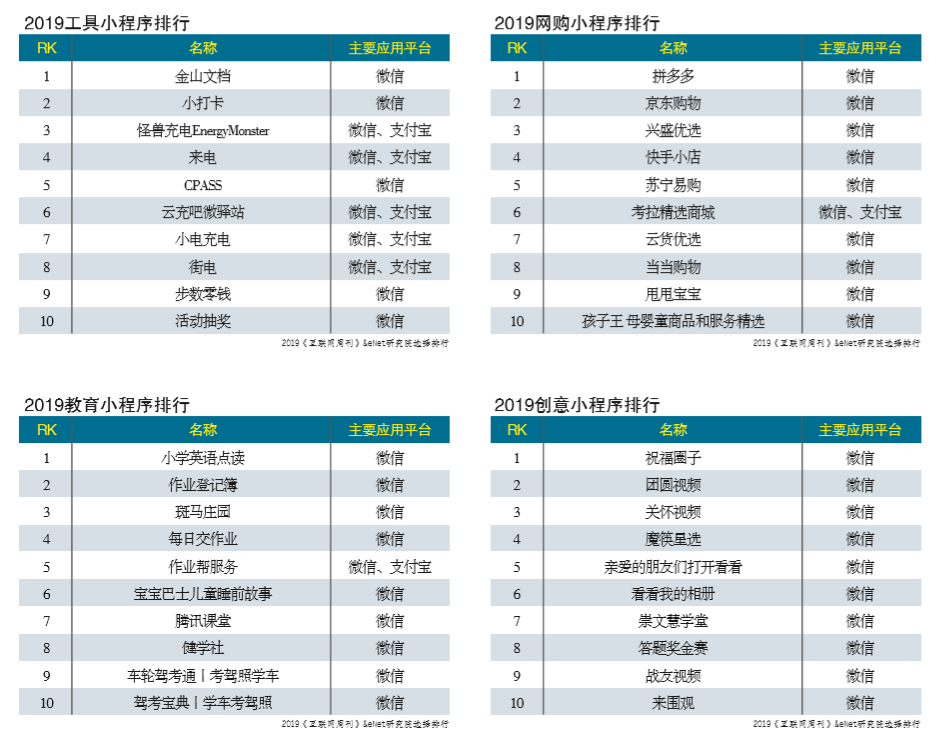
\includegraphics[width=0.7\linewidth]{chart1}
	\caption{2019年度小程序分类排行}
	\label{fig:chart1}
\end{figure}
除微信和支付宝小程序外,百度和头条小程序也越来越活跃。百度在2019 年第二季度财报发布后,李彦宏向百度员工发出了内部信,还特意提到了百度智能小程序的作用,“智能小程序则帮助我们构建起一个新的内容和服务生态。”。同年8月,知乎便宣布完成4.34亿美元F轮融资,百度和快手成了新的投资方。百度表示,将与知乎展开深度战略合作,知乎全站上亿问答将以智能小程序的形式接入百度App,并通过算法分发加入百度搜索、信息流等产品矩阵。\textsuperscript{\citep{caibao}}\par
2018年底,一直被开发者关注的头条小程序终于正式上线。2019年5月初,头条小程序主入口又进行了一次大改版,打造出了一个小程序“应用商店”。就时机而言,今日头条与百度、阿里相比算是比较晚的。头条小程序由于一直处于探索期,一时之间还是让人看不清发展方向,但从最近的布局来看,它的目标应该是“电商和搜索”。\par
虽然小程序目前仍然处于开拓增量市场的阶段,还有非常大的上升与发展空间,但是微信身为小程序概念的创造者已经展现出领袖气质并且优势巨大。支付宝依靠支付宝客户端这一传统的支付工具,在小程序市场也成功分得一杯羹。而百度、字节跳动等其他一众互联网企业也在积极合作、探索。
\subsection{小程序的国外发展}
2019年微信小程序在德国柏林和新加坡办了两场海外开发者大赛,在第二站德国柏林的大赛现场,微信团队公布了公布了一些最新的海外数据:海外小程序的打开速度提升了35\%,日活提升200\%,欧洲地区小程序访问量翻倍;2019年微信支付在境外合规的国家和地区覆盖量增加至60个,支持16种不同货币直接结算。微信也已经上线了小程序英文开发文档、面向服务商的微信开放平台英文介绍页,方便服务商接入并开发小程序。\par
此外,Google公司也有2个类似的免安装服务:Instant App和PWA。Instant App是原生开发的,是类似一个apk的小插件,仅能用于临时使用,没有太大的用处,而且国内的手机厂商也没有引入。而PWA是HTML5的演进,不是原生,它使得网页的能力得到进一步的强化。但是现在看来,Web版应用和PWA其实说的是一回事,因为PWA大部分API已经成为HTML5标准了。微信小程序虽然也是前端技术,但实际上补充了原生扩展能力,包括原生的地图、扫码这些HTML5不具备的能力,也包括补充的原生渲染,比如窗体动画、页面的头尾。另外小程序是典型的客户端应用,不是在线网页。每个小程序都有一个包,是先下载到手机然后解压运行的,只是技术上做了处理,可以变成的非常快。也正式因为小程序做的这些强化,所以小程序的体验要比网页要好,很接近App。\par
虽然微信小程序一直在积极开拓国外市场,并且和一些头部厂商取得了合作。但微信要在海外复制国内的小程序盛况,还需要更多的开发者和服务商加入,去继续做大国外服务市场。
\subsection{小程序的发展前景}
现有的微信小程序在庞大的用户市场上还远没有达到需求 饱和状态,零售业、生活服务业、游戏娱乐业等几个主产业需 求量依然巨大,未来市场将会有更多的小程序被开发和上线。小程序的轻量化和高便利的优势越来越明显。事实上,小程序的分享渠道也在拓宽:关联公众号,制作二维码链接,小程序推送等等。小程序的生态圈进一步完善,程序入口多样化,对于小程序的后期发展非常有益。虽然小程序能够替代部分App,但是缺乏关键功能,用户体验不佳等缺陷是小程序发展的障碍。以微信为例,小程序的开发基于微信平台,这使得开发者不得不牺牲一些创意来跟随微信的开发步伐,而微信所具有的庞大用户群则是明显的优势点。开发者需要权衡利弊,做出自己的选择。
\section{总结}
在此之前,我一直学习的只是小程序的开发技术,没有对小程序的商业模式与发展前景进行太多的研究。通过此门课程,通过研究国内外各大企业对小程序的态度及市场争夺,我不仅对小程序有了更为深刻的认识,还窥得了移动互联网发展的一角。这不禁让我想到了吴军博士曾在《浪潮之巅》\textsuperscript{\citep{lczd}}里写道:近一百多年来,总有一些公司很幸运地、有意无意地站在技术革命的浪尖之上。一旦处在那个位置,即使不做任何事,也可以随着波浪顺顺当当向前漂十年甚至更长的时间。在这十几年到几十年间,它们代表着科技的浪潮,直到下一波浪潮的来临。这些公司里的人,无论职位高低,在外人看来,都是时代的幸运儿。因为,虽然对一个公司来说,赶上一次浪潮不能保证其长盛不衰;但是,对一个人来说,一生赶上一次这样的浪潮就足够了。一个弄潮的年轻人,最幸运的,莫过于赶上一波大潮。\par
这种场面,想想都为之心潮澎湃。而毫无疑问,腾讯、微信、张小龙都是这个时代的弄潮人。从2017 年初微信推出小程序开始,支付宝、百度、今日头条,以 及几大手机厂商都对这种无需下载、即开即用的服务展示了浓厚的兴趣。 在经历短暂的观望之后,已经有越来越多的开发者投身小程序生态中。在人口红利消失、马太效应越来越强的移动互联网世界中,小程序一方面在帮助超级App不断拓展平台边界,另一方面也在帮助开发者获得更多的流量和用户来源,当然对用户来说,寻找内容和获得服务的成本也在降低。\par
总而言之,小程序仅用三年就引起了海量的用户和众多开发者,并且构造起了全新的小程序开发环境和开发者生态。而且市场上升空间巨大,发展前景十分可观。
\par
\section{附录}
\begin{itemize}
    \item GitHub  - https://github.com/GarlicGo
    \begin{figure}[H]
    	\centering
    	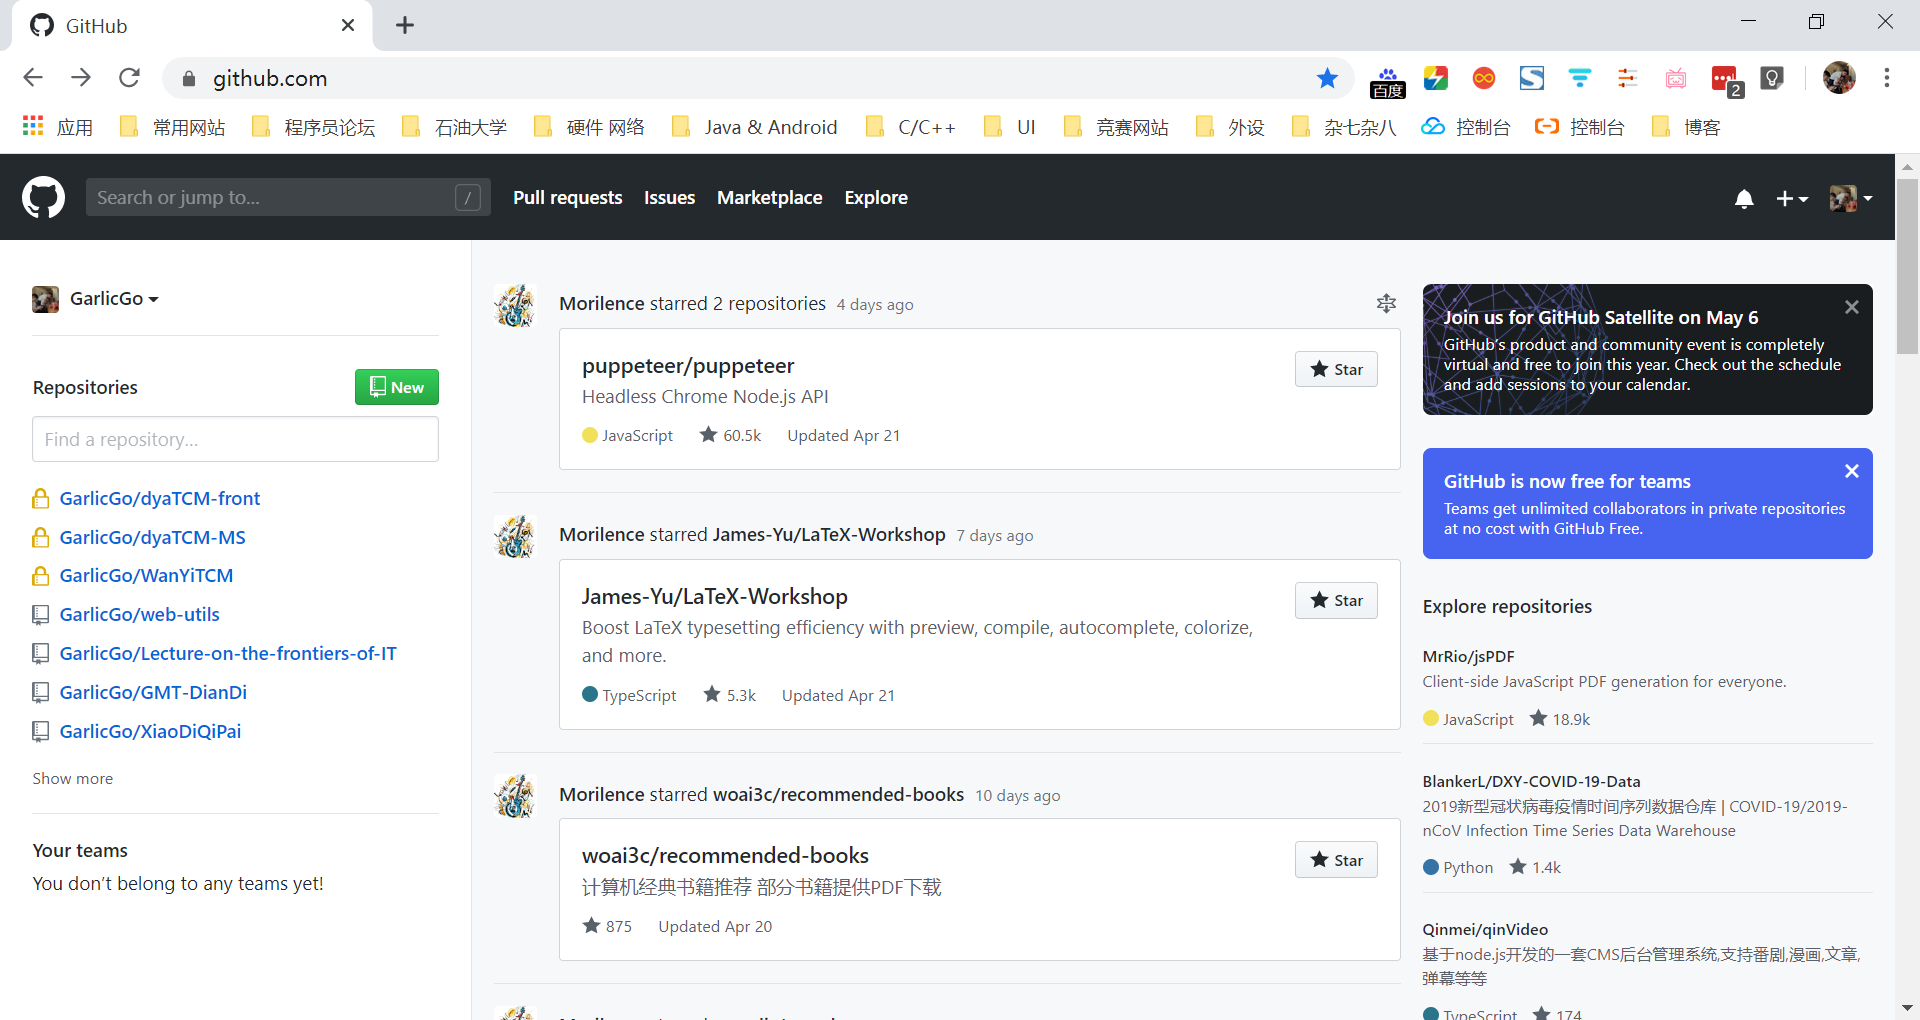
\includegraphics[width=0.7\linewidth]{github1}
    	\caption{GitHub主页}
    	\label{fig:github1}
    \end{figure}
    \begin{figure}[H]
    	\centering
    	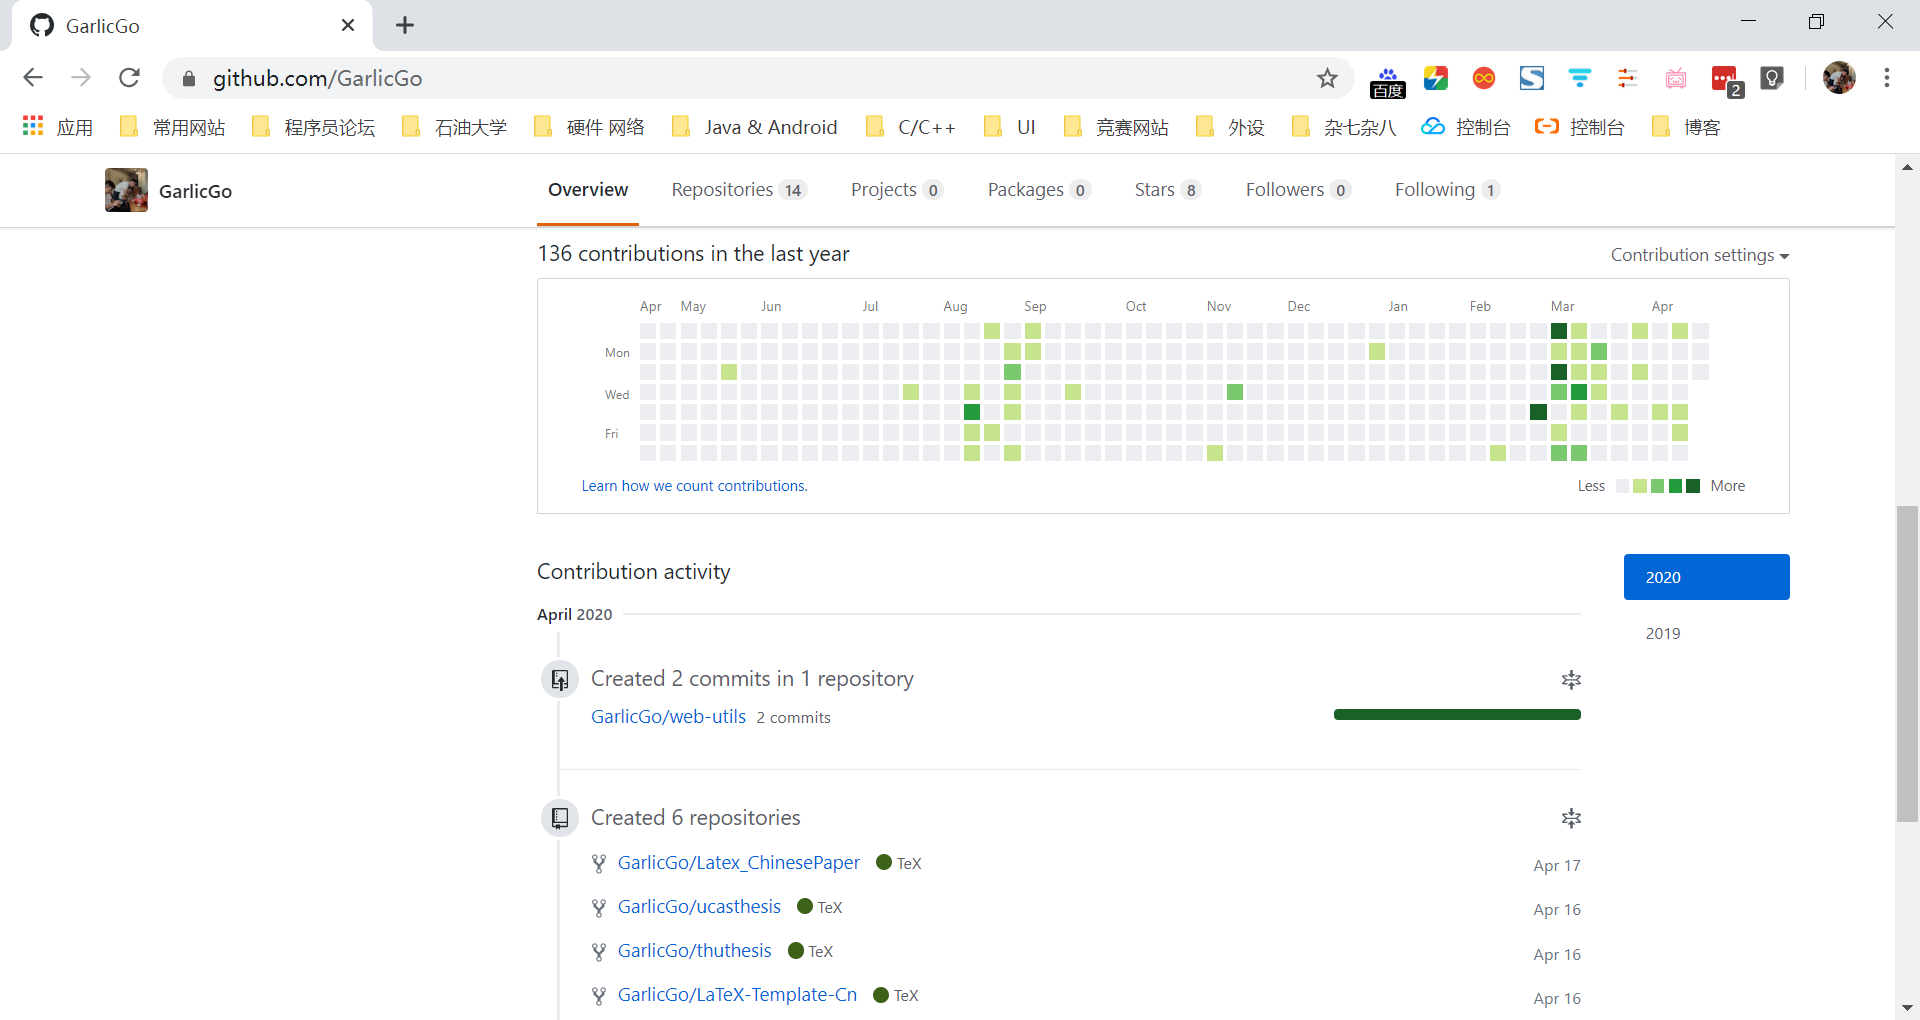
\includegraphics[width=0.7\linewidth]{github2}
    	\caption{profile}
    	\label{fig:github2}
    \end{figure}
	\item 观察者网
	\begin{figure}[H]
		\centering
		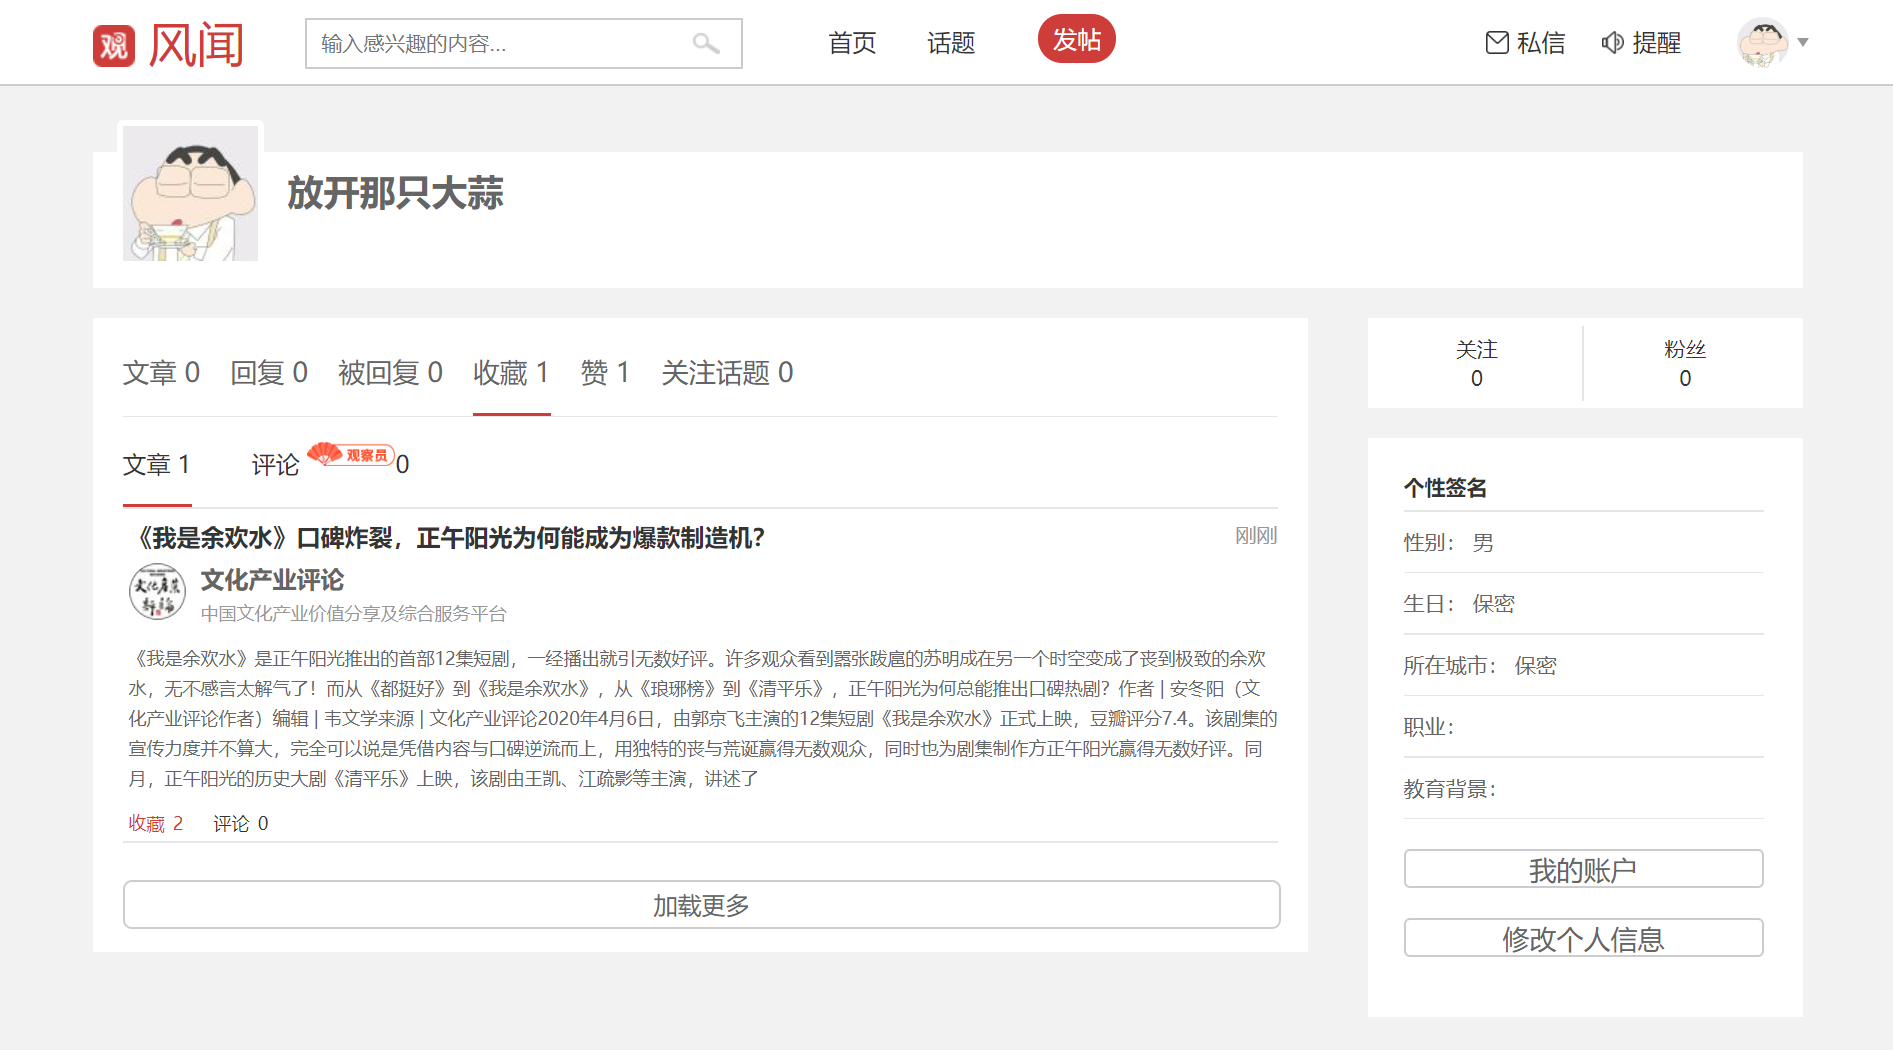
\includegraphics[width=0.7\linewidth]{gczw}
		\caption{观察者网}
		\label{fig:gczw}
	\end{figure}
	\item 学习强国
	\begin{figure}[H]
		\centering
		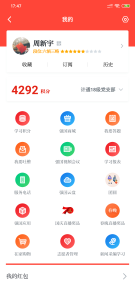
\includegraphics[width=0.3\linewidth]{xxqg}
		\caption{学习强国}
		\label{fig:xxqg}
	\end{figure}
	\item 哔哩哔哩 - https://space.bilibili.com/386323291
	\begin{figure}[H]
		\centering
		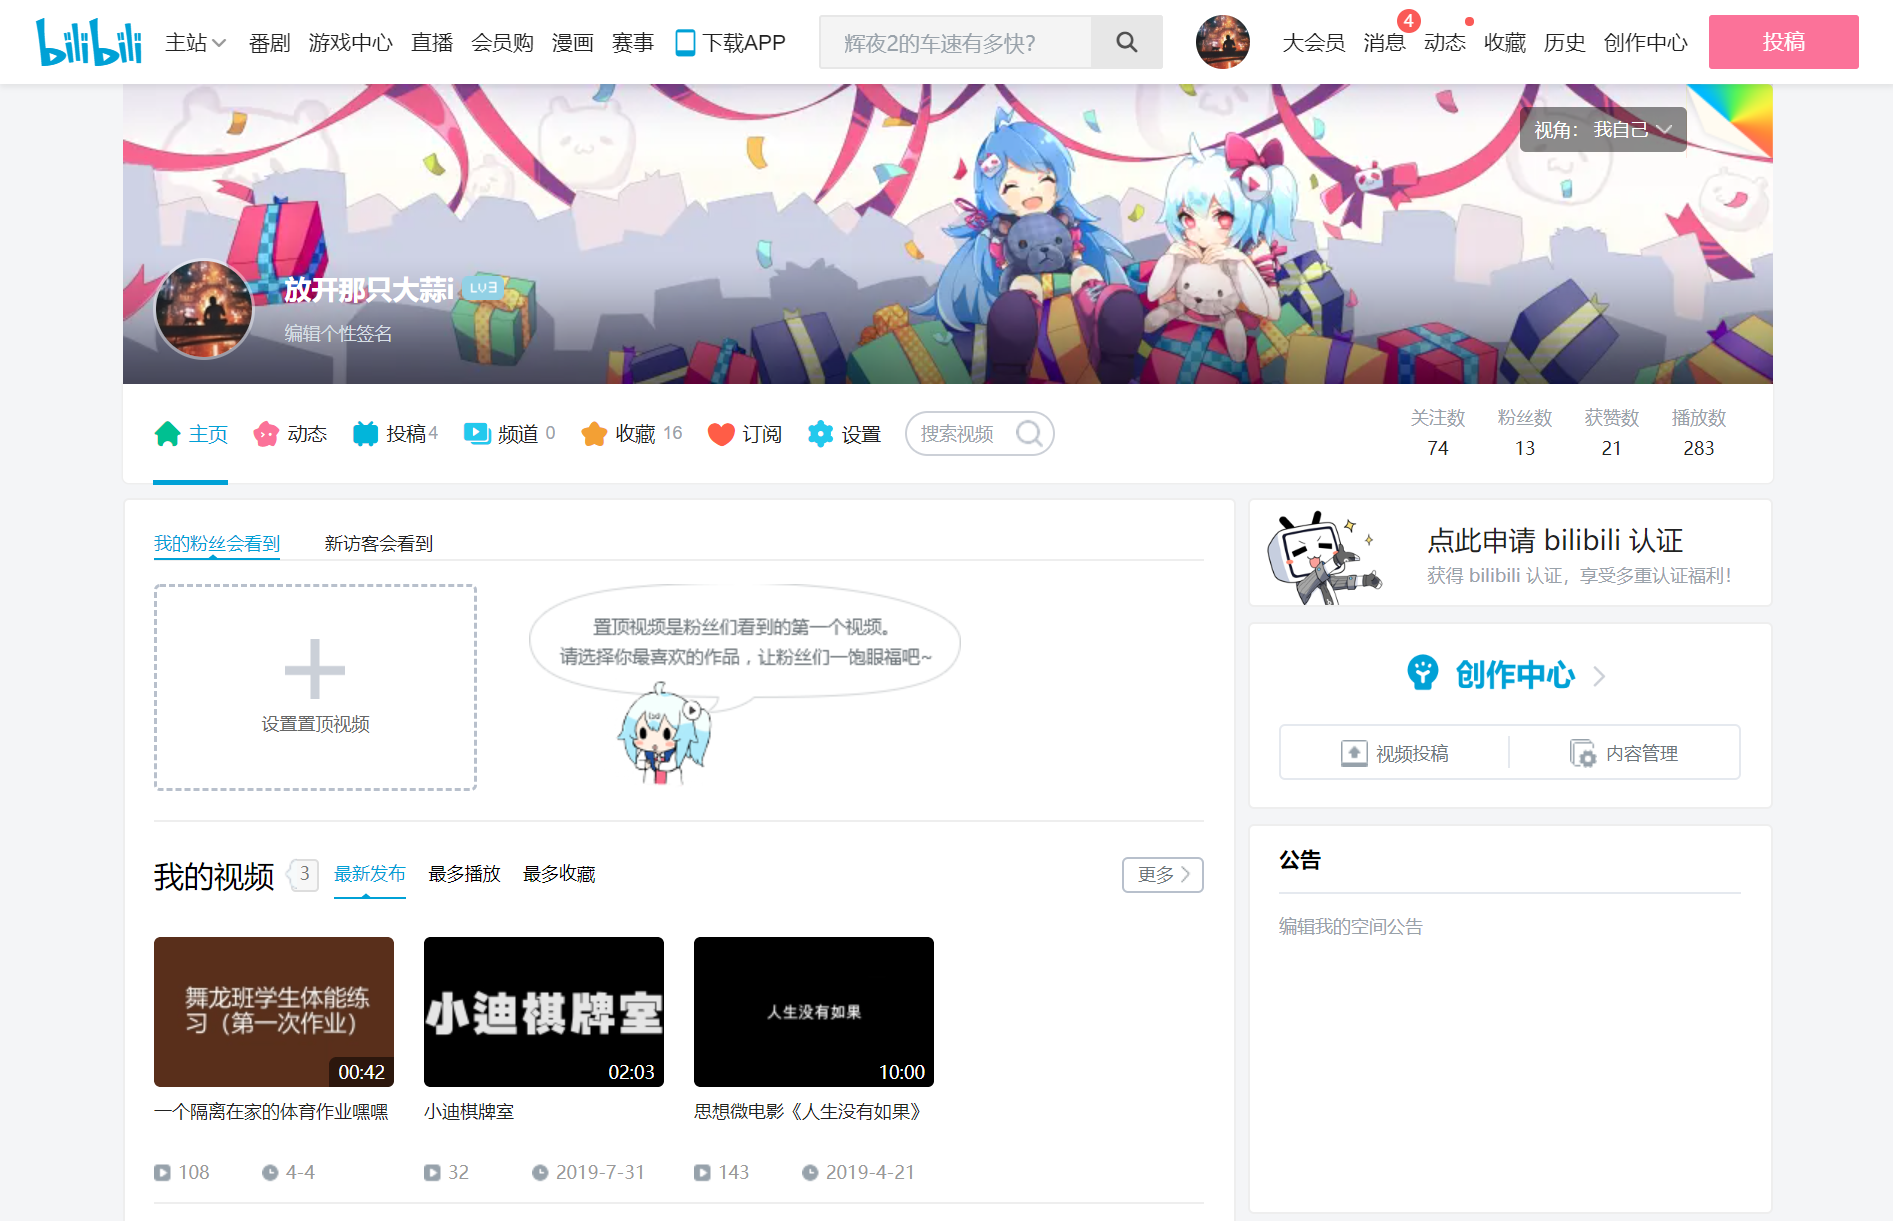
\includegraphics[width=0.7\linewidth]{bilibili}
		\caption{哔哩哔哩}
		\label{fig:bilibili}
	\end{figure}
	\item CSDN - https://me.csdn.net/qq\_43636360
	\begin{figure}[H]
		\centering
		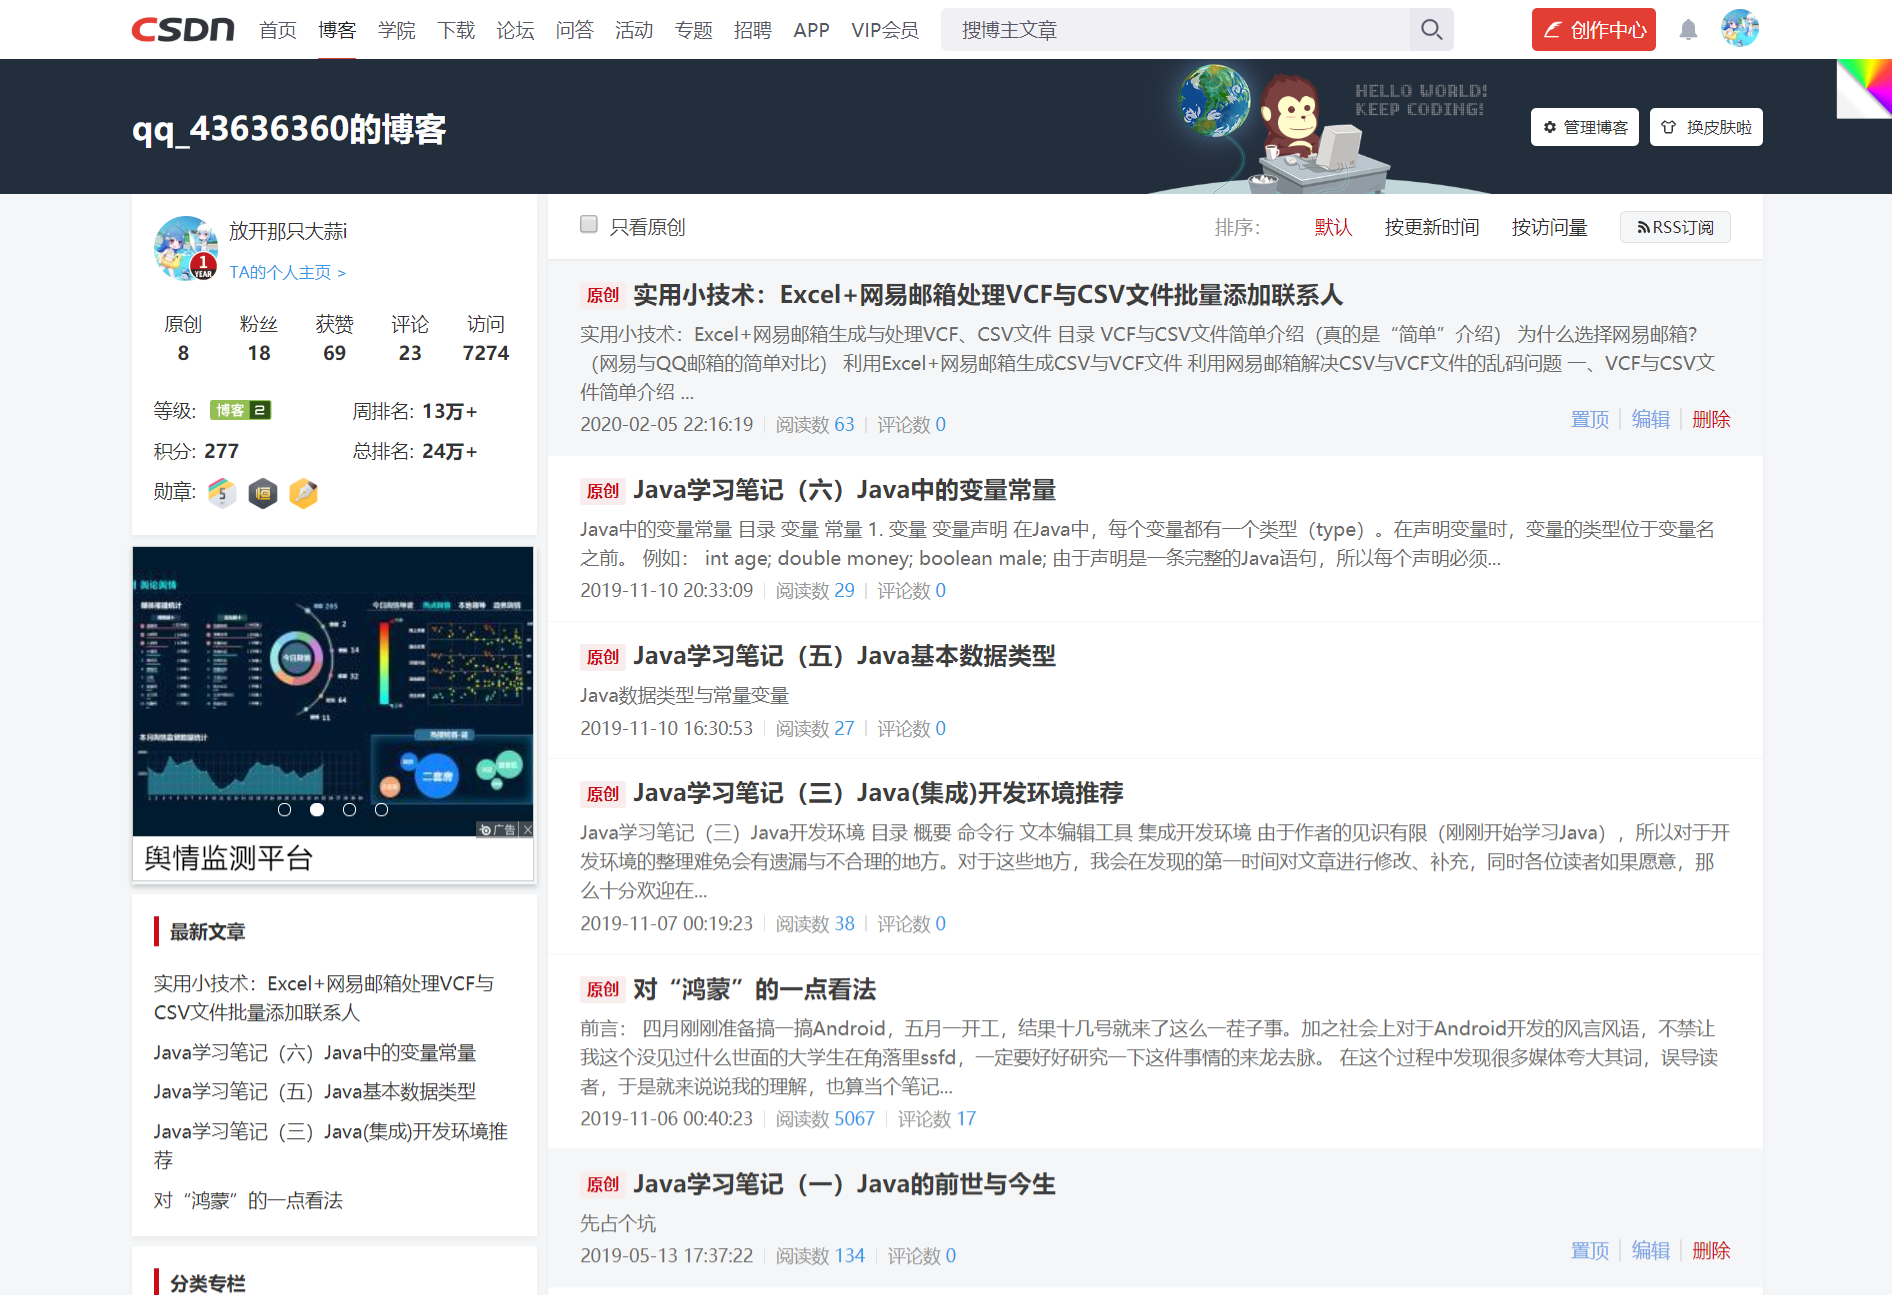
\includegraphics[width=0.7\linewidth]{csdn}
		\caption{CSDN}
		\label{fig:csdn}
	\end{figure}
	\item 博客园 - https://www.cnblogs.com/garlicgo/
	\begin{figure}[H]
		\centering
		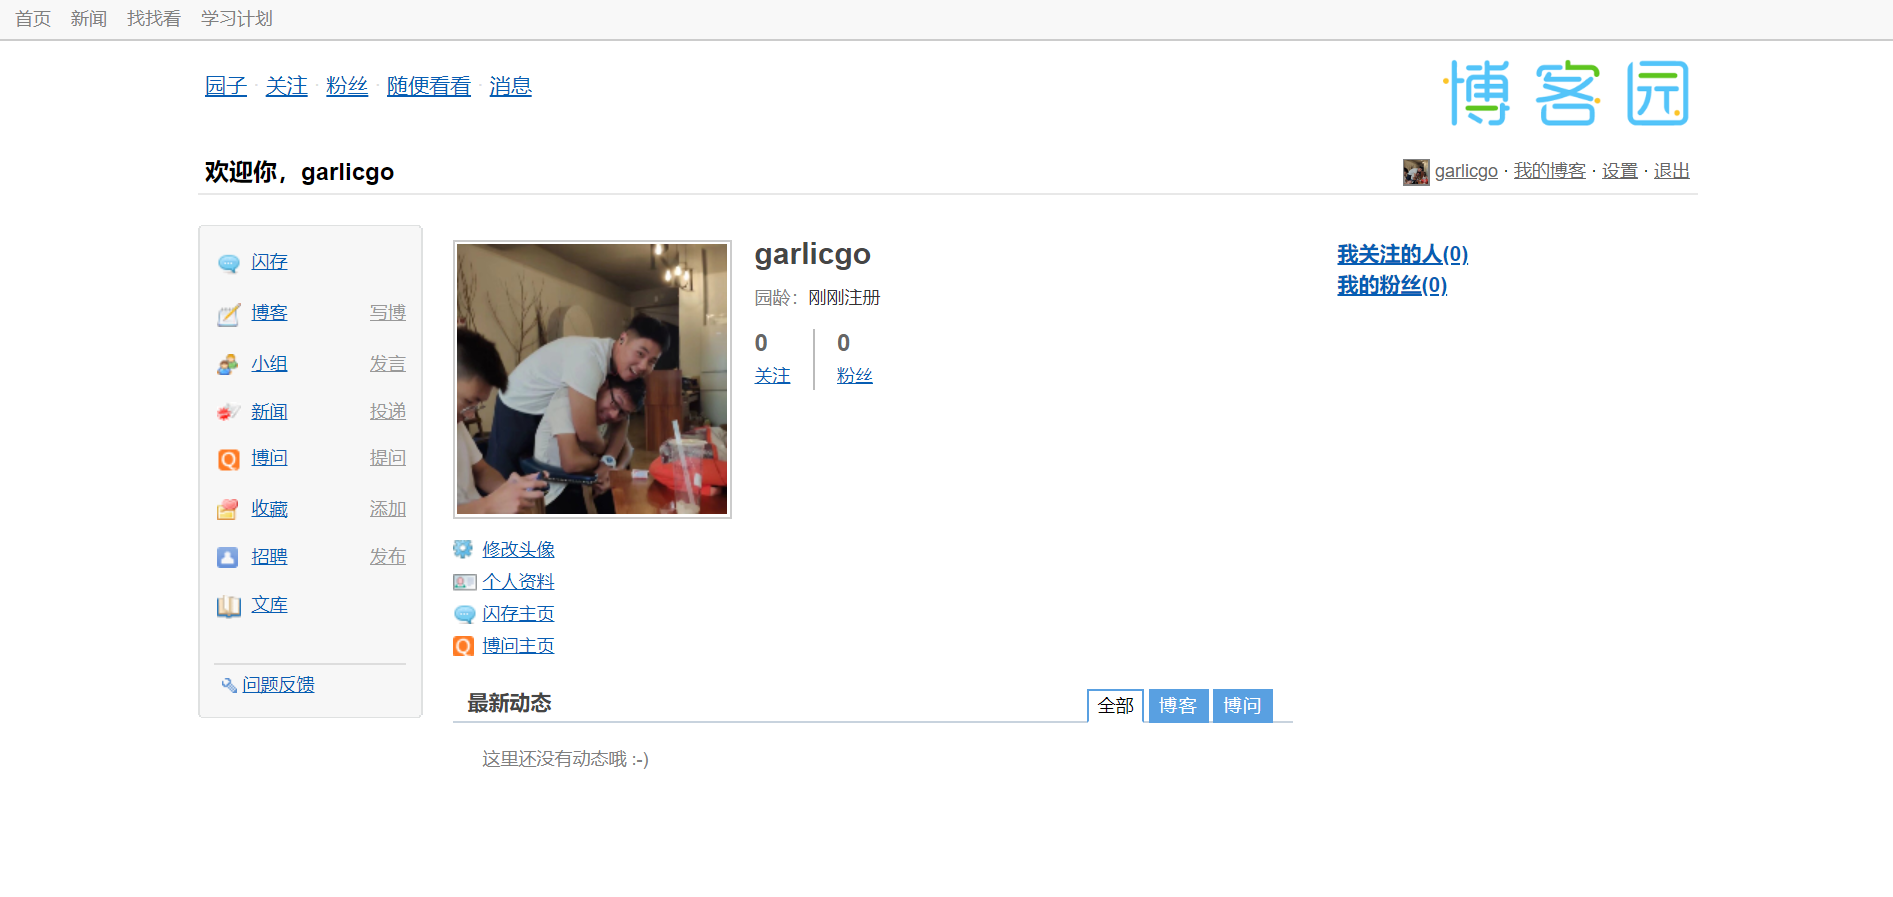
\includegraphics[width=0.7\linewidth]{bky}
		\caption{博客园}
		\label{fig:bky}
	\end{figure}
	\item 小木虫 - http://muchong.com/bbs/space.php?uid=21023505
	\begin{figure}[H]
		\centering
		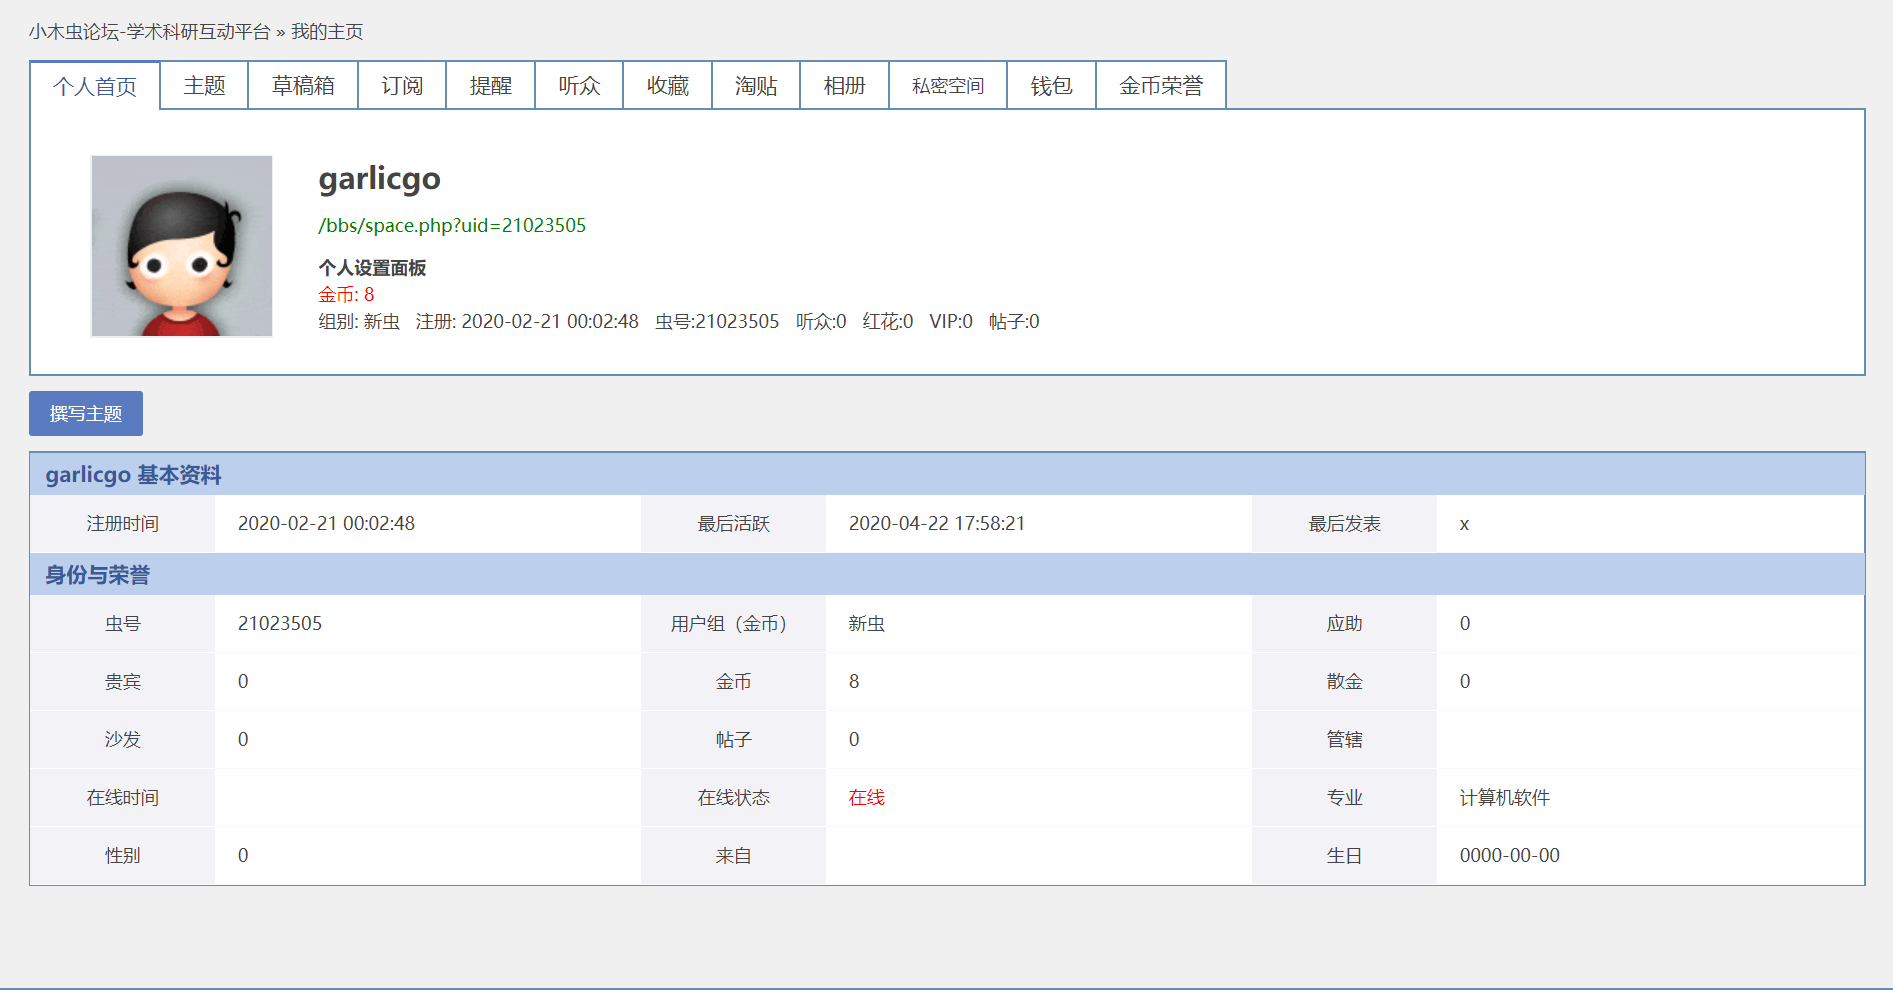
\includegraphics[width=0.7\linewidth]{xmc}
		\caption{小木虫}
		\label{fig:xmc}
	\end{figure}
\end{itemize}


\hspace*{\fill} \\
\bibliographystyle{plain}
\bibliography{references}


\end{document}
